\documentclass{standalone}
\usepackage{tikz}
\usetikzlibrary{decorations.pathreplacing,decorations.pathmorphing}
\usetikzlibrary{fit,quotes}
\usepackage{yquant, braket}

\begin{document}

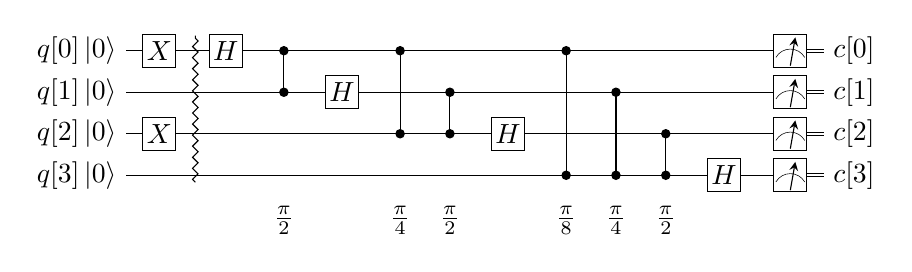
\begin{tikzpicture}[scale=1.000000,x=1pt,y=1pt]
\filldraw[color=white] (0.000000, -7.500000) rectangle (252.000000, 52.500000);
% Drawing wires
% Line 2: q0 W q[0]\ket{0} c[0]
\draw[color=black] (0.000000,45.000000) -- (240.000000,45.000000);
\draw[color=black] (240.000000,44.500000) -- (252.000000,44.500000);
\draw[color=black] (240.000000,45.500000) -- (252.000000,45.500000);
\draw[color=black] (0.000000,45.000000) node[left] {$q[0]\ket{0}$};
% Line 3: q1 W q[1]\ket{0} c[1]
\draw[color=black] (0.000000,30.000000) -- (240.000000,30.000000);
\draw[color=black] (240.000000,29.500000) -- (252.000000,29.500000);
\draw[color=black] (240.000000,30.500000) -- (252.000000,30.500000);
\draw[color=black] (0.000000,30.000000) node[left] {$q[1]\ket{0}$};
% Line 4: q2 W q[2]\ket{0} c[2]
\draw[color=black] (0.000000,15.000000) -- (240.000000,15.000000);
\draw[color=black] (240.000000,14.500000) -- (252.000000,14.500000);
\draw[color=black] (240.000000,15.500000) -- (252.000000,15.500000);
\draw[color=black] (0.000000,15.000000) node[left] {$q[2]\ket{0}$};
% Line 5: q3 W q[3]\ket{0} c[3]
\draw[color=black] (0.000000,0.000000) -- (240.000000,0.000000);
\draw[color=black] (240.000000,-0.500000) -- (252.000000,-0.500000);
\draw[color=black] (240.000000,0.500000) -- (252.000000,0.500000);
\draw[color=black] (0.000000,0.000000) node[left] {$q[3]\ket{0}$};
% Done with wires; drawing gates
% Line 6: q0 X
\begin{scope}
\draw[fill=white] (12.000000, 45.000000) +(-45.000000:8.485281pt and 8.485281pt) -- +(45.000000:8.485281pt and 8.485281pt) -- +(135.000000:8.485281pt and 8.485281pt) -- +(225.000000:8.485281pt and 8.485281pt) -- cycle;
\clip (12.000000, 45.000000) +(-45.000000:8.485281pt and 8.485281pt) -- +(45.000000:8.485281pt and 8.485281pt) -- +(135.000000:8.485281pt and 8.485281pt) -- +(225.000000:8.485281pt and 8.485281pt) -- cycle;
\draw (12.000000, 45.000000) node {$X$};
\end{scope}
% Line 7: q2 X
\begin{scope}
\draw[fill=white] (12.000000, 15.000000) +(-45.000000:8.485281pt and 8.485281pt) -- +(45.000000:8.485281pt and 8.485281pt) -- +(135.000000:8.485281pt and 8.485281pt) -- +(225.000000:8.485281pt and 8.485281pt) -- cycle;
\clip (12.000000, 15.000000) +(-45.000000:8.485281pt and 8.485281pt) -- +(45.000000:8.485281pt and 8.485281pt) -- +(135.000000:8.485281pt and 8.485281pt) -- +(225.000000:8.485281pt and 8.485281pt) -- cycle;
\draw (12.000000, 15.000000) node {$X$};
\end{scope}
\draw[decorate,decoration={zigzag,amplitude=1pt,segment length=4}] (25.000000,-2.500000) -- (25.000000,50.500000);
% Line 8: q0 H
\begin{scope}
\draw[fill=white] (36.000000, 45.000000) +(-45.000000:8.485281pt and 8.485281pt) -- +(45.000000:8.485281pt and 8.485281pt) -- +(135.000000:8.485281pt and 8.485281pt) -- +(225.000000:8.485281pt and 8.485281pt) -- cycle;
\clip (36.000000, 45.000000) +(-45.000000:8.485281pt and 8.485281pt) -- +(45.000000:8.485281pt and 8.485281pt) -- +(135.000000:8.485281pt and 8.485281pt) -- +(225.000000:8.485281pt and 8.485281pt) -- cycle;
\draw (36.000000, 45.000000) node {$H$};
\end{scope}
% Line 9: q0 q1 %% $\frac{\pi}{2}$
\draw (57.000000, -7.500000) node[text width=144pt,below,text centered] {$\frac{\pi}{2}$};
\draw (57.000000,45.000000) -- (57.000000,30.000000);
\filldraw (57.000000, 45.000000) circle(1.500000pt);
\filldraw (57.000000, 30.000000) circle(1.500000pt);
% Line 10: q1 H
\begin{scope}
\draw[fill=white] (78.000000, 30.000000) +(-45.000000:8.485281pt and 8.485281pt) -- +(45.000000:8.485281pt and 8.485281pt) -- +(135.000000:8.485281pt and 8.485281pt) -- +(225.000000:8.485281pt and 8.485281pt) -- cycle;
\clip (78.000000, 30.000000) +(-45.000000:8.485281pt and 8.485281pt) -- +(45.000000:8.485281pt and 8.485281pt) -- +(135.000000:8.485281pt and 8.485281pt) -- +(225.000000:8.485281pt and 8.485281pt) -- cycle;
\draw (78.000000, 30.000000) node {$H$};
\end{scope}
% Line 11: TOUCH
% Line 12: q0 q2 %% $\frac{\pi}{4}$
\draw (99.000000, -7.500000) node[text width=144pt,below,text centered] {$\frac{\pi}{4}$};
\draw (99.000000,45.000000) -- (99.000000,15.000000);
\filldraw (99.000000, 45.000000) circle(1.500000pt);
\filldraw (99.000000, 15.000000) circle(1.500000pt);
% Line 13: q1 q2 %% $\frac{\pi}{2}$
\draw (117.000000, -7.500000) node[text width=144pt,below,text centered] {$\frac{\pi}{2}$};
\draw (117.000000,30.000000) -- (117.000000,15.000000);
\filldraw (117.000000, 30.000000) circle(1.500000pt);
\filldraw (117.000000, 15.000000) circle(1.500000pt);
% Line 14: q2 H
\begin{scope}
\draw[fill=white] (138.000000, 15.000000) +(-45.000000:8.485281pt and 8.485281pt) -- +(45.000000:8.485281pt and 8.485281pt) -- +(135.000000:8.485281pt and 8.485281pt) -- +(225.000000:8.485281pt and 8.485281pt) -- cycle;
\clip (138.000000, 15.000000) +(-45.000000:8.485281pt and 8.485281pt) -- +(45.000000:8.485281pt and 8.485281pt) -- +(135.000000:8.485281pt and 8.485281pt) -- +(225.000000:8.485281pt and 8.485281pt) -- cycle;
\draw (138.000000, 15.000000) node {$H$};
\end{scope}
% Line 15: TOUCH
% Line 16: q0 q3 %% $\frac{\pi}{8}$
\draw (159.000000, -7.500000) node[text width=144pt,below,text centered] {$\frac{\pi}{8}$};
\draw (159.000000,45.000000) -- (159.000000,0.000000);
\filldraw (159.000000, 45.000000) circle(1.500000pt);
\filldraw (159.000000, 0.000000) circle(1.500000pt);
% Line 17: q1 q3 %% $\frac{\pi}{4}$
\draw (177.000000, -7.500000) node[text width=144pt,below,text centered] {$\frac{\pi}{4}$};
\draw (177.000000,30.000000) -- (177.000000,0.000000);
\filldraw (177.000000, 30.000000) circle(1.500000pt);
\filldraw (177.000000, 0.000000) circle(1.500000pt);
% Line 18: q2 q3 %% $\frac{\pi}{2}$
\draw (195.000000, -7.500000) node[text width=144pt,below,text centered] {$\frac{\pi}{2}$};
\draw (195.000000,15.000000) -- (195.000000,0.000000);
\filldraw (195.000000, 15.000000) circle(1.500000pt);
\filldraw (195.000000, 0.000000) circle(1.500000pt);
% Line 19: q3 H
\begin{scope}
\draw[fill=white] (216.000000, -0.000000) +(-45.000000:8.485281pt and 8.485281pt) -- +(45.000000:8.485281pt and 8.485281pt) -- +(135.000000:8.485281pt and 8.485281pt) -- +(225.000000:8.485281pt and 8.485281pt) -- cycle;
\clip (216.000000, -0.000000) +(-45.000000:8.485281pt and 8.485281pt) -- +(45.000000:8.485281pt and 8.485281pt) -- +(135.000000:8.485281pt and 8.485281pt) -- +(225.000000:8.485281pt and 8.485281pt) -- cycle;
\draw (216.000000, -0.000000) node {$H$};
\end{scope}
% Line 20: TOUCH
% Line 21: q0 M
\draw[fill=white] (234.000000, 39.000000) rectangle (246.000000, 51.000000);
\draw[very thin] (240.000000, 45.600000) arc (90:150:6.000000pt);
\draw[very thin] (240.000000, 45.600000) arc (90:30:6.000000pt);
\draw[->,>=stealth] (240.000000, 39.600000) -- +(80:10.392305pt);
% Line 22: q1 M
\draw[fill=white] (234.000000, 24.000000) rectangle (246.000000, 36.000000);
\draw[very thin] (240.000000, 30.600000) arc (90:150:6.000000pt);
\draw[very thin] (240.000000, 30.600000) arc (90:30:6.000000pt);
\draw[->,>=stealth] (240.000000, 24.600000) -- +(80:10.392305pt);
% Line 23: q2 M
\draw[fill=white] (234.000000, 9.000000) rectangle (246.000000, 21.000000);
\draw[very thin] (240.000000, 15.600000) arc (90:150:6.000000pt);
\draw[very thin] (240.000000, 15.600000) arc (90:30:6.000000pt);
\draw[->,>=stealth] (240.000000, 9.600000) -- +(80:10.392305pt);
% Line 24: q3 M
\draw[fill=white] (234.000000, -6.000000) rectangle (246.000000, 6.000000);
\draw[very thin] (240.000000, 0.600000) arc (90:150:6.000000pt);
\draw[very thin] (240.000000, 0.600000) arc (90:30:6.000000pt);
\draw[->,>=stealth] (240.000000, -5.400000) -- +(80:10.392305pt);
% Done with gates; drawing ending labels
\draw[color=black] (252.000000,45.000000) node[right] {$c[0]$};
\draw[color=black] (252.000000,30.000000) node[right] {$c[1]$};
\draw[color=black] (252.000000,15.000000) node[right] {$c[2]$};
\draw[color=black] (252.000000,0.000000) node[right] {$c[3]$};
% Done with ending labels; drawing cut lines and comments
% Done with comments
\end{tikzpicture}
\end{document}
